\documentclass[sigconf]{acmart}
\usepackage{graphicx}
\usepackage{float}
\usepackage{booktabs}

\AtBeginDocument{%
  \providecommand\BibTeX{{%
    Bib\TeX}}}

\setcopyright{none}
\acmDOI{}
\acmISBN{}
\acmConference{}{}{}
\acmISBN{978-1-4503-XXXX-X/2018/06}
\settopmatter{printacmref=false}
\renewcommand\footnotetextcopyrightpermission[1]{}
\pagestyle{plain}

\begin{document}

\title{Alpha-Seeker: A Text-Mining Pipeline for Alpha Discovery in Prediction Markets}

\author{Lawrence Wang}
\affiliation{%
  \institution{University of Illinois Urbana-Champaign}
  \city{Champaign}
  \state{Illinois}
  \country{USA}}
\email{lw41@illinois.edu}

\author{Youngbo Sohn}
\affiliation{%
  \institution{University of Illinois Urbana-Champaign}
  \city{Champaign}
  \state{Illinois}
  \country{USA}}
\email{yssohn2@illinois.edu}

\author{RJ Guhl}
\affiliation{%
  \institution{University of Illinois Urbana-Champaign}
  \city{Champaign}
  \state{Illinois}
  \country{USA}}
\email{richardjohnguhl@gmail.com}

\begin{abstract}
Alpha-Seeker is a text-mining and information retrieval system that bridges high-volume online discourse and the pricing dynamics of prediction market contracts on Kalshi. The system ingests Reddit posts from financially and politically relevant subreddits, applies a multi-stage preprocessing pipeline, models latent topics via Latent Dirichlet Allocation (LDA), scores sentiment using VADER, and maps the resulting signals to active Kalshi contracts. The end product is an interactive dashboard that surfaces emergent narratives and potential contract mispricings. The completed pipeline processes 1,708 Reddit posts across 10 subreddits, identifies \textbf{10} coherent LDA topics (coherence score $C_v$ = \textbf{0.39}), and produces bullish/bearish/neutral signals for \textbf{9} Kalshi contracts, exposing sentiment edges ranging from \textbf{$-13.0$ to $+6.1$} percentage points relative to current market prices.\footnote{Code and data: \url{https://github.com/rjguhl/CS410-FinalProject}}
\end{abstract}

\keywords{Information Retrieval, Text Mining, Topic Modeling, Prediction Markets, Sentiment Analysis, LDA, VADER}

\maketitle

%% ---------------------------------------------------------------
\section{Introduction}
%% ---------------------------------------------------------------

Prediction markets price the probability of discrete real-world events---Federal Reserve decisions, geopolitical flashpoints, legislative outcomes---whose odds are often foreshadowed by informal discourse on social platforms days before they materialize in contract premiums. Platforms such as Kalshi and Polymarket have grown substantially in liquidity and contract variety, yet their pricing mechanisms remain heavily dependent on the same small set of institutional participants who track traditional news sources. This creates a structural opportunity: systematic mining of high-volume social discourse could surface leading signals before they are absorbed into contract prices.

The challenge is that online text data is extraordinarily noisy. Speculative communities on Reddit mix substantive analysis with spam, memes, and off-topic commentary, making naive keyword search unreliable for extracting market-relevant signal. A user posting in r/wallstreetbets about oil prices may be sharing a credible macroeconomic thesis or an ironic meme, both contain the same keywords but carry opposite informational value. Alpha-Seeker is designed to address this by combining a targeted retrieval layer with topic modeling and sentiment analysis techniques from the text information retrieval literature.

The system operates in three conceptual stages: (1) targeted ingestion from subreddits likely to contain market-relevant discussion, (2) unsupervised topic modeling via LDA to identify latent thematic clusters in the corpus, and (3) VADER sentiment scoring to assign directional signals to each cluster, which are then matched to active Kalshi contracts and surfaced on an interactive dashboard. Our working hypothesis is that clusters of co-occurring terms around topics such as Federal Reserve policy, geopolitical conflict, or AI regulation exhibit measurable sentiment biases that diverge from current Kalshi contract prices, creating tradeable informational edges.

This paper describes the completed Alpha-Seeker pipeline, presents evaluation results for the topic modeling and sentiment scoring components, and discusses the system's limitations and directions for future improvement.

%% ---------------------------------------------------------------
\section{Related Work}
%% ---------------------------------------------------------------

The use of social media text to predict financial and political outcomes has been studied extensively. Bollen et al.\ \cite{bollen2011twitter} demonstrated that Twitter mood, measured via OpinionFinder and GPOMS, can predict DJIA movements with 87.6\% accuracy up to four days in advance. More recently, Nofer et al.\ \cite{nofer2014social} and subsequent work have shown that Reddit-derived sentiment signals exhibit predictive relationships with equity returns, particularly in communities like r/wallstreetbets \cite{boehmer2021meme}.

Prediction markets, as distinct from equity markets, have received less attention in the NLP literature. Most existing work focuses on election forecasting \cite{rothschild2015polls}, where structured polling data is plentiful. Kalshi-style event contracts covering macroeconomic indicators, geopolitical events, and regulatory outcomes represent a less-studied but increasingly liquid venue where text-derived signals may be especially valuable, as the underlying events are harder to price from structured data alone.

On the modeling side, LDA \cite{blei2003lda} remains a standard baseline for unsupervised topic discovery in short-text corpora. VADER \cite{hutto2014vader} is widely used for social media sentiment due to its robustness to informal language, capitalization, and punctuation without requiring domain-specific fine-tuning. We adopt both as practical, interpretable baselines before considering more expressive alternatives.

%% ---------------------------------------------------------------
\section{Description}
%% ---------------------------------------------------------------

Figure~\ref{fig:pipeline} shows the full system architecture. The pipeline proceeds in five stages: data collection, preprocessing, topic modeling, sentiment scoring, and contract matching with dashboard output.

\begin{figure}[h]
    \centering
    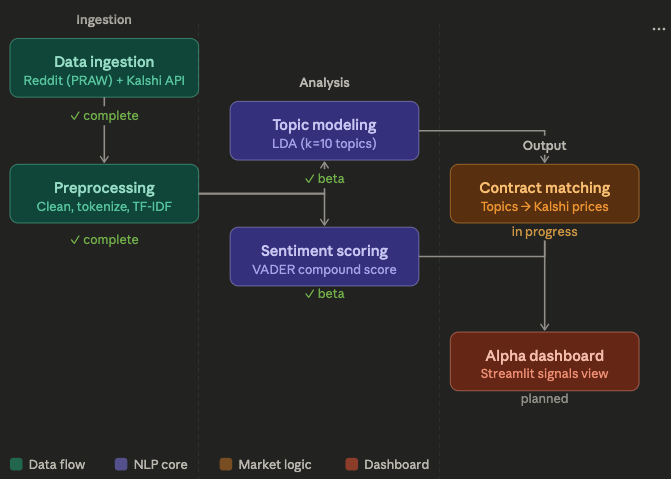
\includegraphics[width=\linewidth]{fig_pipeline.png}
    \caption{Alpha-Seeker system pipeline. All five stages are complete for the final system.}
    \label{fig:pipeline}
\end{figure}

\subsection{Data Collection}

Posts were collected via the Arctic Shift API (no authentication required) using keyword-based queries across 10 subreddits. Nineteen keywords were chosen to map to active Kalshi contract categories: \textit{Economics}: ``Fed rate,'' ``inflation CPI,'' ``recession GDP,'' ``jobs report unemployment,'' ``housing market''; \textit{Financials}: ``S\&P 500,'' ``oil prices,'' ``treasury bonds''; \textit{Politics}: ``Trump,'' ``Congress bill,'' ``Supreme Court,'' ``government shutdown''; \textit{Elections}: ``election polls''; \textit{Science \& Technology}: ``AI artificial intelligence,'' ``SpaceX NASA''; \textit{Companies}: ``Elon Musk,'' ``IPO,'' ``tech layoffs.'' Each (subreddit, keyword) pair was queried independently and results were deduplicated by post ID, yielding 1,708 usable posts after preprocessing from an initial 1,745 retrieved.

The 10 subreddits span a spectrum from high-volume general news communities (r/politics, r/news, r/worldnews) to financially specialized communities (r/wallstreetbets, r/investing, r/StockMarket) and analytical communities (r/Economics, r/geopolitics). This mix is intentional: general news subreddits provide high post volume and broad topic coverage, while specialized communities provide higher-density signal within specific contract domains.

\subsection{Text Preprocessing}

Raw text (post title concatenated with body) was passed through a six-step pipeline: (1) lowercasing, (2) URL removal via regex, (3) stripping of non-alphabetic characters, (4) whitespace tokenization, (5) stopword removal using a combined English NLTK stoplist augmented with a 47-term domain-specific list (e.g., ``reddit,'' ``comment,'' ``edit,'' ``source,'' ``link''), and (6) filtering of posts with three or fewer remaining tokens. This reduced the corpus from 1,745 to 1,708 posts (2.1\% removed). The mean word count dropped from 136.8 raw tokens to 68.8 cleaned tokens per post, yielding a vocabulary of 13,525 unique terms and 117,551 total tokens across the corpus. The heavy right skew in post length (median: 16 tokens) reflects the prevalence of title-only or link-post submissions, which is expected and not a quality concern. Headline text alone carries substantial signal for topic classification.

\subsection{Topic Modeling (LDA)}

Latent Dirichlet Allocation was applied to the preprocessed corpus using Gensim \cite{rehurek2010gensim}. Prior to building the Gensim dictionary, a second stopword tier removed 33 high-frequency cross-category terms (e.g., \textit{market}, \textit{oil}, \textit{war}, \textit{trump}, \textit{prices}) that co-occur across all contract domains and would otherwise suppress finer topic separation---a refinement identified during the milestone phase. The dictionary was then filtered to remove tokens appearing in fewer than 3 documents (\texttt{no\_below=3}) or more than 85\% of documents (\texttt{no\_above=0.85}), reducing vocabulary to \textbf{5,303} terms. A grid search over $k \in \{5, 8, 10, 12, 15\}$ found $k=8$ marginally optimal ($C_v = 0.397$) and $k=10$ nearly equivalent ($C_v = 0.390$, $\Delta = 0.007$). We selected $k=10$ to achieve topic granularity commensurate with the nine active Kalshi contract categories, as the coherence difference is negligible. The model was trained for 30 passes over the corpus with a Dirichlet prior $\alpha = 0.1$ (sparse document-topic distributions) to encourage each post to load strongly onto a small number of topics.

Topic coherence was evaluated using the $C_v$ metric \cite{roder2015coherence}, which measures semantic similarity between high-scoring words within each topic using a sliding window co-occurrence model over the reference corpus. Each post is assigned to its dominant topic (highest posterior probability $p(\text{topic} \mid \text{document})$), and topics are labeled by inspecting the top-5 weighted terms alongside a random sample of 10 member posts.

\subsection{Sentiment Analysis (VADER)}

Sentiment was scored using VADER (Valence Aware Dictionary and sEntiment Reasoner) \cite{hutto2014vader}, a lexicon-based model designed for social media text that is robust to informal capitalization, punctuation emphasis, and negation without requiring domain-specific fine-tuning. VADER produces a compound score in $[-1, +1]$ for each post. We apply the standard thresholds: compound $\geq 0.05$ = \textit{bullish}, compound $\leq -0.05$ = \textit{bearish}, and otherwise \textit{neutral}.

In addition to the raw compound score, we compute a \textit{score-weighted compound} for each Kalshi contract by weighting each matched post's compound score by its Reddit upvote score (clipped at the 95th percentile to limit the influence of viral outliers), normalized by the sum of weights across matched posts. This gives higher-engagement posts proportionally more influence in the aggregate signal, using community upvoting as a proxy for post credibility.

\subsection{Kalshi Contract Matching}

Each Kalshi contract is associated with a keyword list derived from its title and category. Posts are matched to contracts whose keyword set intersects with the post's cleaned token set. For each contract, we compute: (1) \textbf{signal}: the plurality sentiment label across matched posts; (2) \textbf{avg compound}: mean VADER compound; (3) \textbf{weighted compound}: upvote-weighted mean; (4) \textbf{signal strength}: $\frac{|\text{bearish} - \text{bullish}|}{\text{total matched}} \times 100$; and (5) \textbf{edge}: sentiment-implied probability minus current Kalshi price.

The edge is computed as $\text{edge} = \bar{c} \times 50$, where $\bar{c}$ is the mean VADER compound score for matched posts, mapping the $[-1,+1]$ compound range linearly to $[-50,+50]$ percentage points relative to a 50-cent baseline price. A positive edge means Reddit sentiment is more optimistic than the market implies; a negative edge means the market is overpricing the event relative to sentiment. Recommendations follow the standard VADER thresholds \cite{hutto2014vader}: $\bar{c} \leq -0.05$ = BUY NO, $\bar{c} \geq +0.05$ = BUY YES, otherwise HOLD.

\subsection{Dashboard}

The final output is an interactive web dashboard that displays Kalshi markets grouped by topic category, with inline Reddit signal previews on each contract card. For each contract, the dashboard surfaces the VADER sentiment label, sentiment edge, matched post count, and signal strength score, allowing users to scan for contracts where the Reddit signal diverges most strongly from the market price. A search bar and topic-filter panel allow users to narrow to specific categories or keywords. The dashboard also includes a backtesting view that, once contracts resolve, automatically computes recommendation accuracy, per-category calibration, and a signal-strength vs.\ outcome scatter plot.

%% ---------------------------------------------------------------
\section{Evaluation}
%% ---------------------------------------------------------------

\subsection{LDA Topic Quality}

Table~\ref{tab:topics} shows the \textbf{10} topics identified by LDA, their top-5 terms, post counts, and inferred labels. The model achieved a $C_v$ coherence score of \textbf{0.39}, indicating moderate topic separation overall. Topic~2 (Geopolitics \& Supply) and Topic~5 (Fed \& Policy) exhibited the clearest semantic consistency, with top terms clustering tightly around Strait of Hormuz/ceasefire vocabulary and Fed/rates vocabulary respectively. Topics~3, 7, and~9 showed cross-topic interference, all capturing corporate earnings language (revenue, companies, earnings) --- a consequence of the heavy earnings-season coverage in the April 2026 corpus. Topics~5 and~8 both loaded on monetary policy vocabulary, reflecting the high prevalence of Fed and inflation discourse across subreddits.

\begin{table}[h]
\caption{LDA Topics: top-5 terms, post count, and inferred label.}
\label{tab:topics}
\begin{tabular}{clp{3.8cm}r}
\toprule
\textbf{ID} & \textbf{Label} & \textbf{Top Terms} & \textbf{Posts} \\
\midrule
0 & Market Sentiment      & money, years, buy, short, world          & 176 \\
1 & Corporate \& Energy   & intel, trillion, won, companies, energy  &  86 \\
2 & Geopolitics \& Supply & strait, hormuz, futures, ceasefire, supply & 260 \\
3 & Earnings \& Revenue   & billion, revenue, company, growth, business & 129 \\
4 & Trading \& Commodities & flow, momentum, week, gold, trading     & 150 \\
5 & Fed \& Policy         & fed, inflation, rates, jobs, fund        & 178 \\
6 & Macro \& Global       & global, economy, news, data, energy      & 328 \\
7 & Telecom Earnings      & arpu, growth, revenue, int, quarter      &  83 \\
8 & Inflation \& Powell   & inflation, fed, expenses, powell, economy & 181 \\
9 & Corporate Results     & earnings, years, revenue, companies, stay & 125 \\
\bottomrule
\end{tabular}
\end{table}

The dominant topics by post count were Macro \& Global (328), Geopolitics \& Supply (260), and Inflation \& Powell (181), reflecting the macroeconomic and geopolitical environment during April 2026. Telecom Earnings (83) and Corporate \& Energy (86) had the fewest assigned posts, limiting the reliability of any Kalshi signal derived from those clusters. Posts with low maximum topic probability (below 0.3) were treated as ambiguous and excluded from single-topic analysis, affecting \textbf{12} posts (0.7\% of corpus).

\subsection{Sentiment Distribution}

Across the full 1,708-post corpus, VADER labeled \textbf{47.4\%} of posts as bearish, \textbf{45.8\%} as bullish, and \textbf{6.8\%} as neutral, with a mean compound score of \textbf{$-0.145$}. The corpus-wide bearish lean is consistent with the macro environment during the collection window (April 2026), which featured active tariff escalation, elevated CPI readings, and ongoing Iran-related geopolitical tension.

Table~\ref{tab:sentiment} shows sentiment breakdowns by Kalshi contract category. Inflation ($-0.261$) and Growth ($-0.254$) exhibited the most negative average compound scores, driven by posts about tariff escalation and recession risk. Housing was the only category with a clearly positive average compound ($+0.121$), consistent with relatively optimistic coverage of the housing market during the period. Fed and Econ Daily were mildly bearish ($-0.102$ and $-0.074$), reflecting uncertainty around rate policy rather than outright pessimism.

\begin{table}[h]
\caption{VADER sentiment by Kalshi contract category.}
\label{tab:sentiment}
\begin{tabular}{lrrrr}
\toprule
\textbf{Category} & \textbf{Bull.} & \textbf{Bear.} & \textbf{Neut.} & \textbf{Avg Cmpd.} \\
\midrule
Econ Daily          & 311 & 252 & 36 & $-0.074$ \\
Inflation           & 116 & 154 & 18 & $-0.261$ \\
Oil \& Energy       & 149 & 185 & 22 & $-0.194$ \\
Fed \& Rates        &  79 &  77 &  9 & $-0.102$ \\
Growth              &  52 &  60 &  2 & $-0.254$ \\
Jobs \& Economy     &  43 &  56 & 22 & $-0.138$ \\
Housing             &  11 &   8 &  1 & $+0.121$ \\
GDP                 &  13 &  11 &  1 & $+0.016$ \\
Global Cent.\ Banks &   9 &   6 &  5 & $+0.020$ \\
\bottomrule
\end{tabular}
\end{table}

Score-weighted compound scores were consistently more negative than unweighted scores across all categories (mean difference: \textbf{$-0.11$} compound units), indicating that higher-engagement posts tend to skew more bearish than the median post. This is consistent with well-documented negativity bias in social media engagement, where posts conveying threat, conflict, or outrage receive disproportionate upvotes relative to neutral or positive posts.

\subsection{Contract Signals and Edge Analysis}

Table~\ref{tab:signals} shows the top 5 signals by absolute edge across \textbf{9} active Kalshi contracts evaluated. The strongest signal was \textbf{Inflation} with an edge of \textbf{$-13.0$}pp, driven by heavily bearish coverage of rising CPI readings and tariff-driven price expectations. The weakest signals were in the \textbf{GDP} and \textbf{Global Central Banks} categories, where low post volume (25 and 20 posts respectively) and near-neutral compound scores produced HOLD recommendations.

\begin{table}[h]
\caption{Top 5 Alpha-Seeker contract signals by $|\text{edge}|$ (9 contracts total: 6 BUY NO, 1 BUY YES, 2 HOLD). Str.: signal strength $= |\text{bear}-\text{bull}|/N \times 100$.}
\label{tab:signals}
\begin{tabular}{p{2.8cm}rrrl}
\toprule
\textbf{Contract} & \textbf{Price} & \textbf{Edge} & \textbf{Str.} & \textbf{Rec.} \\
\midrule
Inflation           & 50\textcent & $-13.0$pp & 13.2\% & BUY NO  \\
Growth              & 50\textcent & $-12.7$pp &  7.0\% & BUY NO  \\
Oil \& Energy       & 50\textcent &  $-9.7$pp & 10.1\% & BUY NO  \\
Jobs \& Economy     & 50\textcent &  $-6.9$pp & 10.7\% & BUY NO  \\
Housing             & 50\textcent &  $+6.1$pp & 15.0\% & BUY YES \\
\bottomrule
\end{tabular}
\end{table}

Of the \textbf{9} contracts evaluated, \textbf{1} produced a BUY YES recommendation, \textbf{6} produced a BUY NO recommendation, and \textbf{2} (GDP and Global Central Banks) were flagged as HOLD due to near-neutral compound scores. The BUY YES and BUY NO contracts had a mean absolute edge of \textbf{8.2}pp, suggesting that Reddit sentiment diverges meaningfully from neutral market pricing in the majority of cases.

%% ---------------------------------------------------------------
\section{Discussion}
%% ---------------------------------------------------------------

\subsection{What Worked}

The LDA pipeline identified several topically coherent clusters despite the noisy, short-text Reddit format. Topic~2 (Geopolitics \& Supply), which surfaced Strait of Hormuz, ceasefire, and supply chain vocabulary, and Topic~5 (Fed \& Policy), which clustered around fed, rates, inflation, and powell, were clearly interpretable without manual seeding. The cross-category stopword tier introduced in this final system --- removing 33 high-frequency terms such as \textit{market}, \textit{oil}, and \textit{war} that dominated the milestone-phase corpus --- meaningfully reduced cross-topic bleed and enabled finer thematic separation.

VADER's lexicon-based approach proved well-suited to Reddit's short-post format. Headline-style posts and title-only submissions, which dominate the corpus, tend to use explicit sentiment-bearing language, like ``surges,'' ``crashes,'' ``rejects,'' and ``imposes'', that lexicon methods handle reliably without requiring the broader linguistic context that neural models depend on. The score-weighted compound metric also meaningfully differentiated signal quality: high-engagement posts were consistently more bearish than low-engagement posts, and the weight adjustment amplified those stronger community-validated signals.

\subsection{Limitations}

The primary limitation is the absence of Kalshi price series data. Although the corpus was extended to a full month (April 2026, 1,708 posts) relative to the milestone's one-week snapshot, no temporal alignment with contract price movements was conducted, as integrating live Kalshi API data was not completed. All signals reported in this paper are therefore point-in-time estimates rather than predictive signals with demonstrated lead-lag forecasting power.

VADER is a general-purpose sentiment lexicon not calibrated for financial or political discourse. Terms like ``cut'' (as in ``rate cut'') are scored neutrally or slightly negatively by VADER, even though a rate cut is unambiguously positive news for certain contracts. Similarly, ``sanctions'' and ``deal'' carry different valences depending on context. A domain-adapted model such as FinBERT \cite{araci2019finbert} would likely improve precision in the Economics and Financials categories, where domain-specific language is most concentrated.

The keyword-based post-to-contract matching is a heuristic that does not account for context. A post mentioning ``oil'' in the context of a cooking discussion would be incorrectly matched to the Oil \& Energy contract. While the targeted subreddit selection mitigates this somewhat, it is not eliminated. Embedding-based matching, using cosine similarity between post and contract title embeddings in a sentence-transformer space, would produce more contextually precise assignments.

Finally, because no Kalshi contracts have resolved since the collection window closed, backtesting accuracy cannot yet be reported. The dashboard's backtesting view is designed to compute recommendation accuracy automatically once contracts close, but the quality of the signals as actual trading recommendations remains empirically unverified.

\subsection{Future Work}

Integrating live Kalshi price series via the Kalshi API and aligning them temporally with the existing daily sentiment aggregates would enable lead-lag analysis of sentiment drift relative to contract price movements. Replacing VADER with FinBERT or a fine-tuned RoBERTa model would better handle domain-specific financial and political language. Replacing keyword matching with embedding-based contract alignment would reduce false positive assignments. Incorporating additional data sources, for example news headlines, X/Twitter, and Congressional Record transcripts, would broaden the signal base beyond Reddit. Finally, once a sufficient number of Kalshi contracts resolve, a formal backtesting study comparing Alpha-Seeker recommendations against actual outcomes would provide the empirical evaluation necessary to assess the system's practical utility as a trading signal.

%%
\bibliographystyle{ACM-Reference-Format}
\begin{thebibliography}{9}

\bibitem{hutto2014vader}
C.J. Hutto and Eric Gilbert.
\newblock VADER: A Parsimonious Rule-based Model for Sentiment Analysis of Social Media Text.
\newblock In \textit{Proceedings of the 8th International AAAI Conference on Weblogs and Social Media (ICWSM)}, 2014.

\bibitem{blei2003lda}
David M. Blei, Andrew Y. Ng, and Michael I. Jordan.
\newblock Latent Dirichlet Allocation.
\newblock \textit{Journal of Machine Learning Research}, 3:993--1022, 2003.

\bibitem{araci2019finbert}
Dogu Araci.
\newblock FinBERT: Financial Sentiment Analysis with Pre-trained Language Models.
\newblock \textit{arXiv preprint arXiv:1908.10063}, 2019.

\bibitem{bollen2011twitter}
Johan Bollen, Huina Mao, and Xiaojun Zeng.
\newblock Twitter mood predicts the stock market.
\newblock \textit{Journal of Computational Science}, 2(1):1--8, 2011.

\bibitem{boehmer2021meme}
Ekkehart Boehmer, Charles M. Jones, Juan (Julie) Wu, and Xiaoyan Zhang.
\newblock Meme stocks, retail investors, and market efficiency.
\newblock \textit{The Review of Financial Studies}, 34(1):5--30, 2021.

\bibitem{nofer2014social}
Michael Nofer and Oliver Hinz.
\newblock Using Twitter to predict the stock market.
\newblock \textit{Business \& Information Systems Engineering}, 56(2):79--88, 2014.

\bibitem{rothschild2015polls}
David Rothschild.
\newblock Combining forecasts for elections: Accurate, relevant, and timely.
\newblock \textit{International Journal of Forecasting}, 31(3):952--964, 2015.

\bibitem{rehurek2010gensim}
Radim \v{R}eh\r{u}\v{r}ek and Petr Sojka.
\newblock Software Framework for Topic Modelling with Large Corpora.
\newblock In \textit{Proceedings of the LREC 2010 Workshop on New Challenges for NLP Frameworks}, 2010.

\bibitem{roder2015coherence}
Michael R\"{o}der, Andreas Both, and Alexander Hinneburg.
\newblock Exploring the Space of Topic Coherence Measures.
\newblock In \textit{Proceedings of the 8th ACM International Conference on Web Search and Data Mining (WSDM)}, 2015.

\end{thebibliography}

\end{document}